%% V1.0
%% by Ussama Naal, usa.naal@gmail.com
%% Trying to be Udacious!

\documentclass[10pt,journal,compsoc]{IEEEtran}

\usepackage[pdftex]{graphicx}    
\usepackage{cite}
\usepackage{fullpage}
\usepackage{times}
\usepackage{fancyhdr,graphicx,amsmath,amssymb}
\usepackage[ruled,vlined]{algorithm2e}
\usepackage{url}
\include{pythonlisting}
\hyphenation{op-tical net-works semi-conduc-tor}


\begin{document}

\title{ROS AMCL Robot Navigation}

\author{Ussama Naal}

\markboth{Paricles Filter, Robotic Nanodegree, Udacity}%
{}
\IEEEtitleabstractindextext{%

\begin{abstract}
In this work we investigate the use an MCL variant algorithm known as AMCL. We do this within a simulated environment using ROS and Gazebo. We setup a two wheeled robot with a map that has a given track. The robot is then equipped with a rangefinder and an odometer to track the robot motion. We then feed the readings from these sensors to AMCL ros package and let it control the robot. With a bit of tuning for the parameters of AMCL and other ros packages the the robot can successfully navigate to the target goal.
\end{abstract}

% Note that keywords are not normally used for peerreview papers.
\begin{IEEEkeywords}
Robot navigation, ROS, particle filter, MCL, AMCL.
\end{IEEEkeywords}}


\maketitle
\IEEEdisplaynontitleabstractindextext
\IEEEpeerreviewmaketitle
\section{Introduction}
\label{sec:introduction}

\IEEEPARstart To carry out a successful robot navigation within a given world or map, the robot must be able to locate itself within that map. For this, robots are typically equipped with multiple sensors such as cameras, laser scanners, odometers, etc. These sensors help the robot identify its surrounding area as it moves through out the map. For example, laser scanners give the robot a measurement of how far obstacles like walls are from the robot. An odometer tracks the path that robot is moving along from the initial pose.

\begin{figure}[thpb]
      \centering
      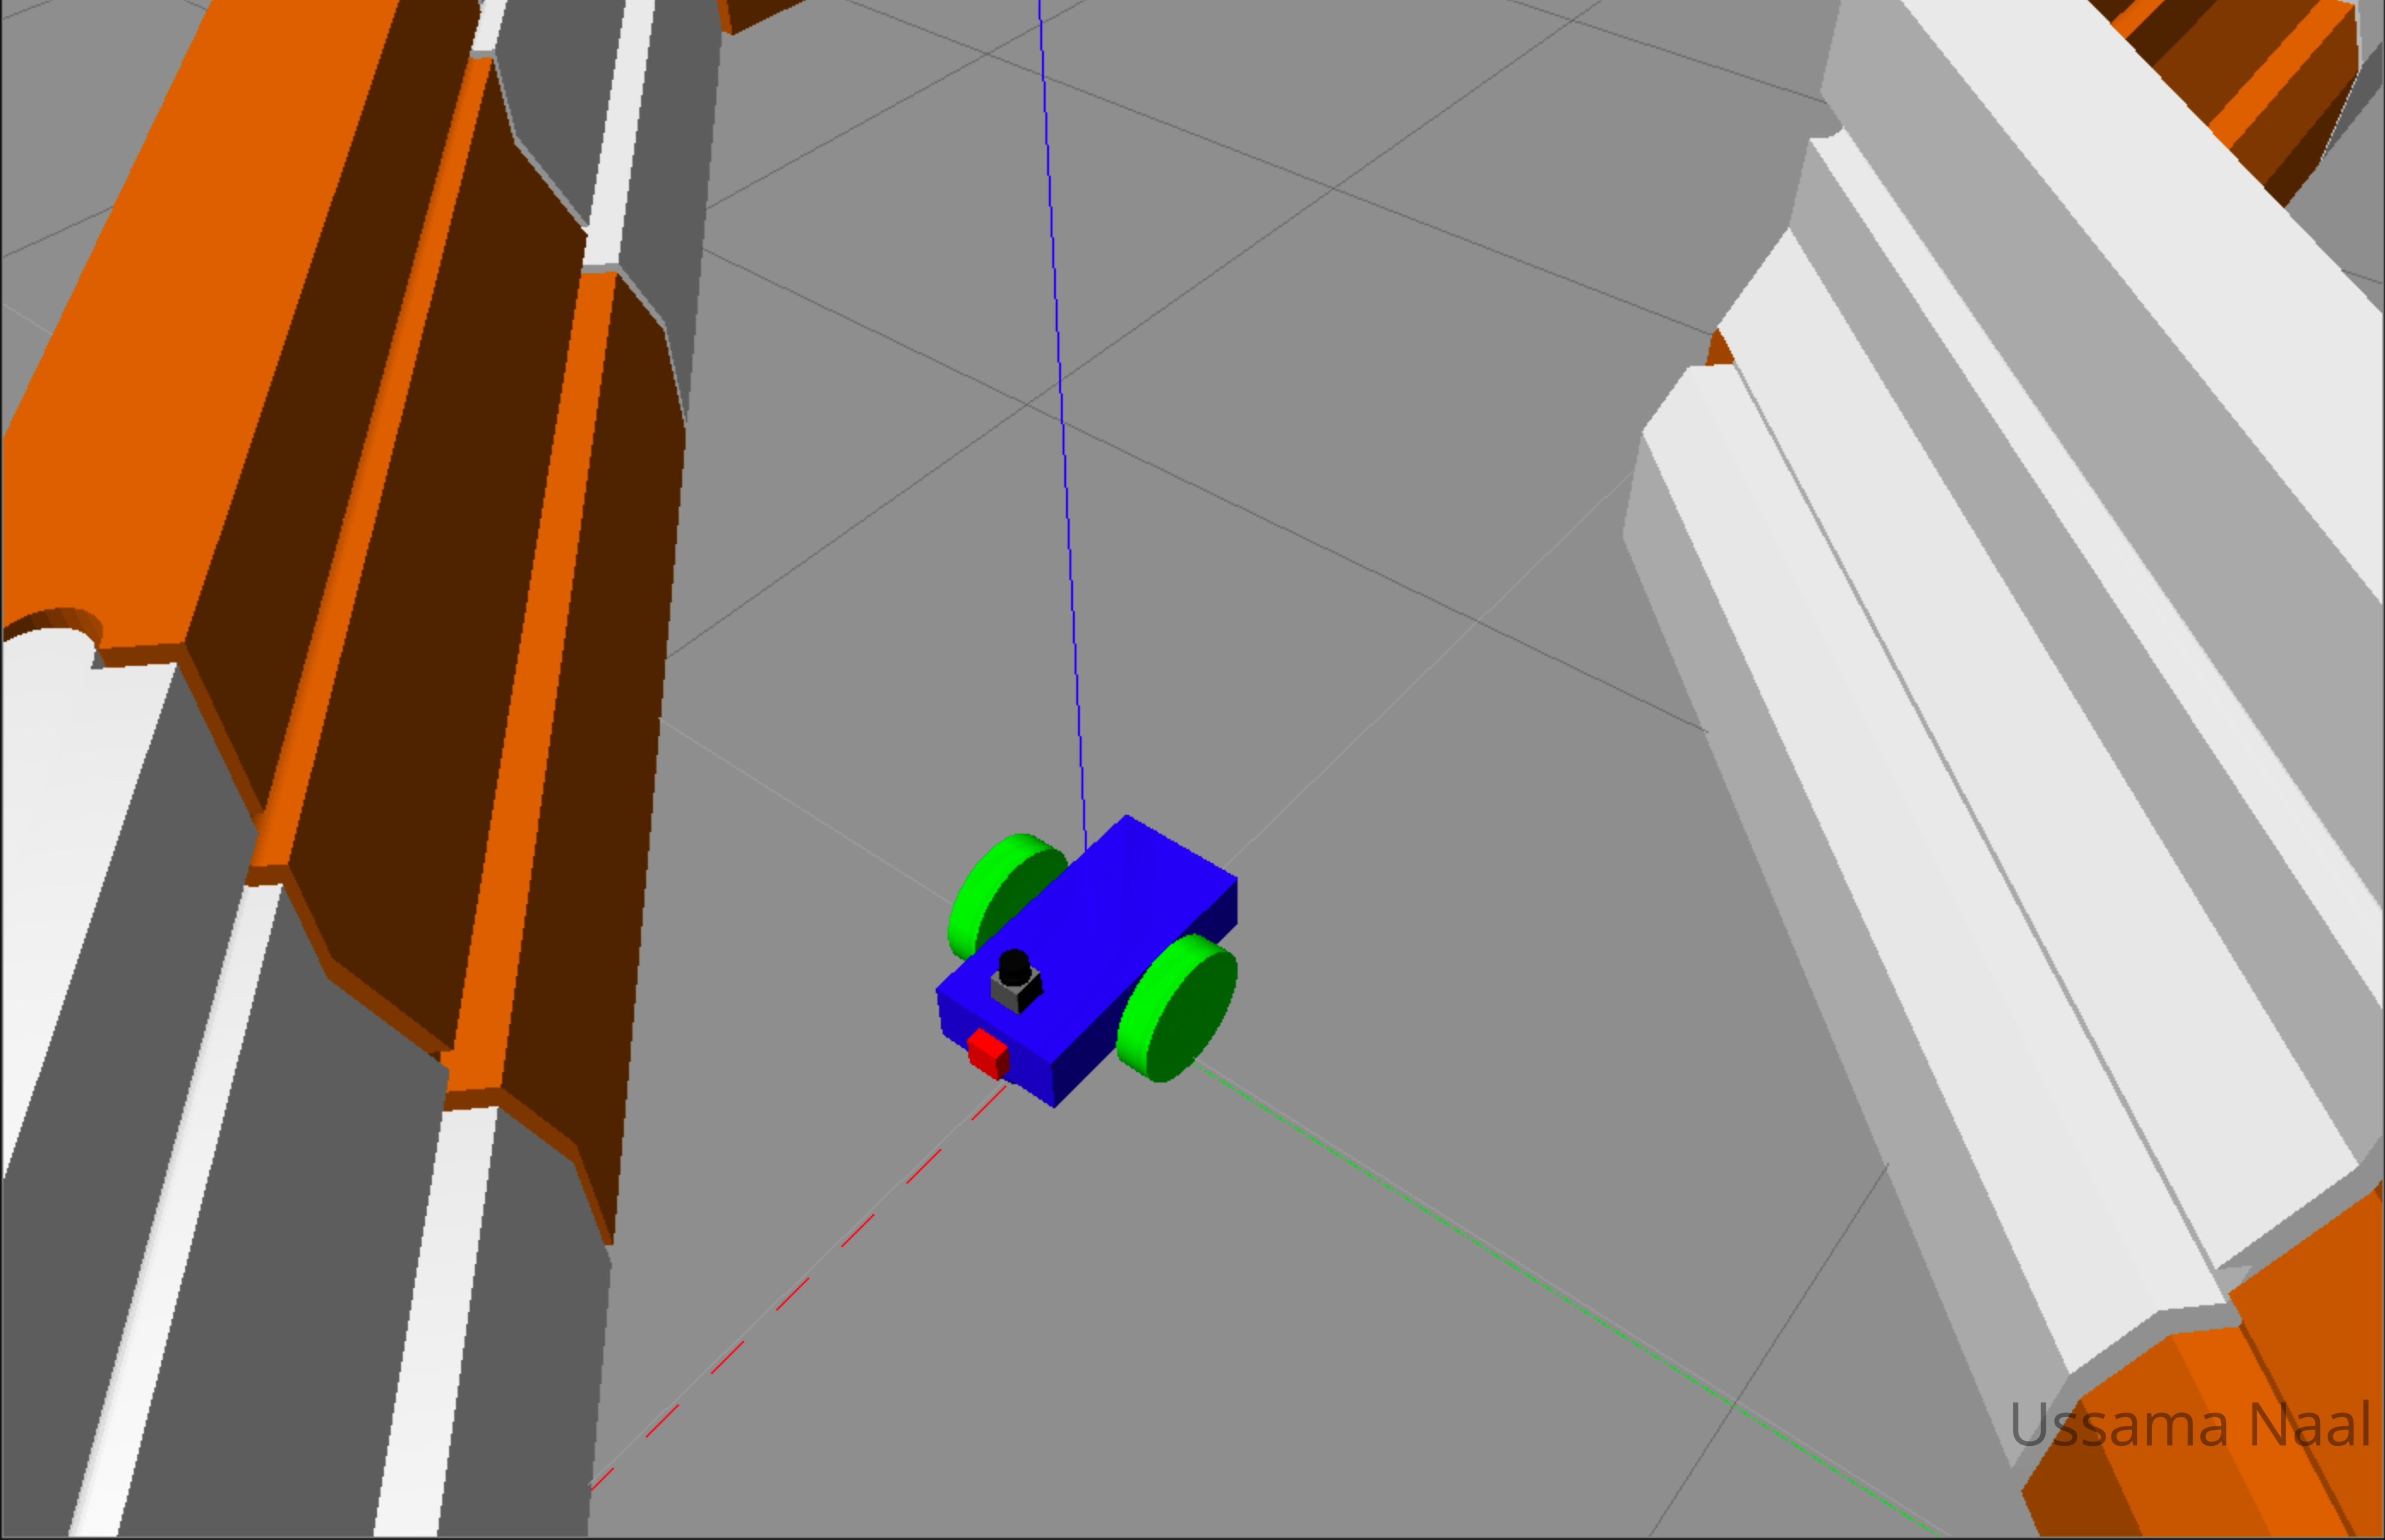
\includegraphics[width=\linewidth]{robot-image.png}
      \caption{Image of our test robot.}
      \label{fig:cnn-classifier}
\end{figure}

\section{Background / Formulation}
As mentioned, the sensors provide the robot with measurements that can help the robot estimate its position within the map. However, the measurements supplied by the sensors may not be fully accurate due to noise. Kalman filters can reduce the impact of the noise on the measurements if the noise has a Gaussian distribution and the system is linear. Extended Kalman Filters can work for system that are non-linear in nature but still requires the noise to follow a Gaussian distribution. However, when this is not the case a better alternative would be to employ MCL or Particles Filter. Particles filter work for non-linear systems and doesn't require that noise coming from sensor measurements to have a Gaussian distribution.

The following listing shows the basic steps in the MCL algorithm:

\begin{algorithm}
\SetAlgoLined
\caption{MCL Algorithm}
\SetKwFunction{FMCL}{MCL}
\SetKwProg{Fn}{Function}{:}{\KwRet{$X_t$}}
\Fn{\FMCL{$X_{t-1}$, $u_t$, $z_t$}}{
    $\bar{X_t} = X_t = {\phi}$\;
    \For {m=1 to M}{
        $X_t^{[m]} = motion\_update(u_t, x_{t-1}^{[m]})$;
        $w_t^{[m]} = sensor\_update(z_t, x_t^{[m]})$;
        $\bar{X_t} = \bar{X_t} + < x_t^{[m]}, w_t^{[m]} >$;
    }
    \For {m=1 To M} {
        Draw $X_t^{[m]}$ from $\bar{X_t}$ with probability \propto $w_t^{[m]}$;
        $X_t = X_t^{[m]}$;
    }
}
\end{algorithm}

\section{Model Configuration}
Our robot is composed of a main chassis and two large side wheels. To help keep the robot stable we add two caster wheels at the front and the back of the robot as shown below:
\begin{figure}[thpb]
      \centering
      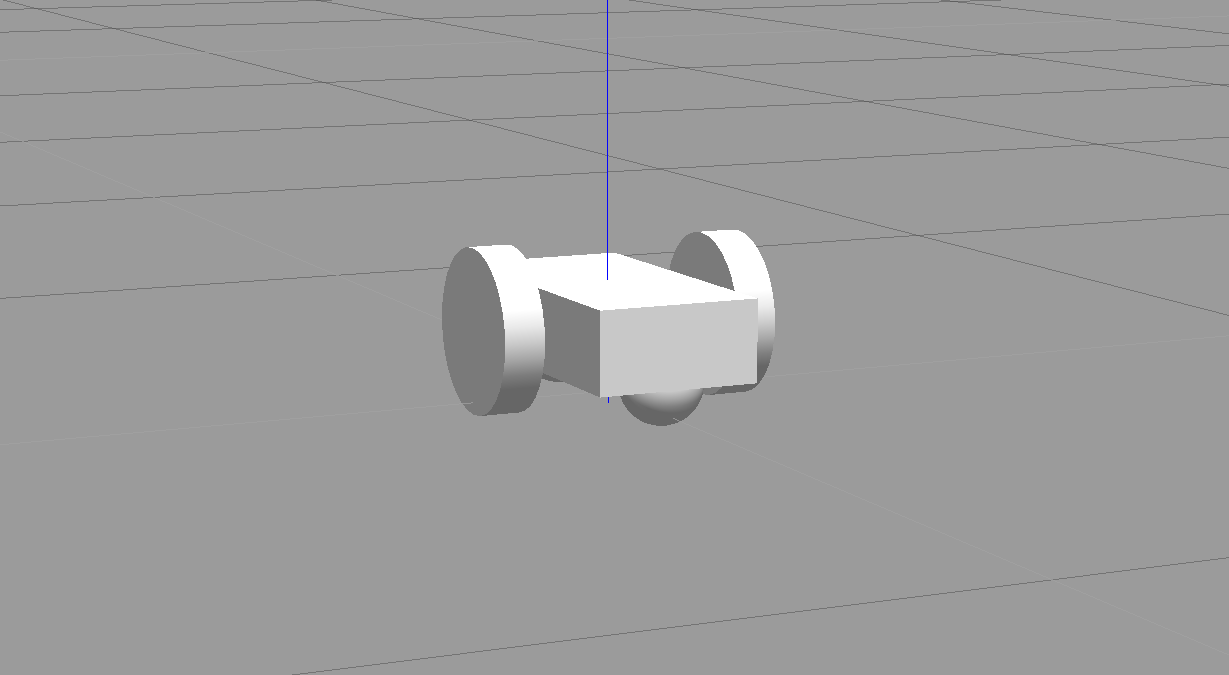
\includegraphics[width=\linewidth]{gazebo-robot.png}
      \caption{Robot Setup.}
      \label{fig:network-training}
\end{figure}

We also equip the robot with a camera at the front of the robot which allows us the see what the robot might be facing while it moves. We place a Hokuyo rangefinder on the top of the robot at the front. The rangefinder measures how far obstacles are from the robot.

Then we enable AMCL ROS package which will guide the robot to a target goal. The AMCL package implements an adaptive version of the MCL algorithm, where the algorithm changes the number of samples used in real-time \cite{what-is-amcl}. Once the robot localizes itself, lower number of samples is required to do the tracking. The advantages of this is a better of efficiency for the robot, and also allows the robot stay responsive with measurements that come from sensors at a higher rate \cite{Fox99montecarlo}.

The following table lists parameters to make the simulation functioning within the system used to run the simulation:

\begin{table}[h]
\caption{Simulation Update Parameters}
\label{table_example}
\begin{center}
\begin{tabular}{|c||c|}
\hline
Parameter & Value\\
\hline
transform\_tolerance & 0.2 \\
\hline
update\_frequency (Local) & 14 Hz \\
\hline
publish\_frequency (Local) & 14 Hz\\
\hline
update\_frequency (Global) & 14 Hz \\
\hline
publish\_frequency (Global) & 14 Hz \\
\hline
controller\_update & 14 Hz \\
\hline
\end{tabular}
\end{center}
\end{table}

Setting these values is important to have the simulation proceed with no issues or warnings reported on the console.

Next we configure another set of parameters for the costmap as shown in Table 2.
\begin{table}[h]
\caption{Costmap Parameters}
\label{table_example}
\begin{center}
\begin{tabular}{|c||c|}
\hline
Parameter & Value\\
\hline
inflation\_radius & 0.7 \\
\hline
inflation\_radius & 0.5 \\
\hline
raytrace\_range & 4.0 \\
\hline
\end{tabular}
\end{center}
\end{table}

These parameters tune the costmap such that it prevents the robot from getting stock against walls or other obstacles on the map.

Finally, we tweak some of the parameters for the AMCL package \cite{ros-amcl} as shown in Table 3.
\begin{table}[h]
\caption{AMCL Parameters}
\label{table_example}
\begin{center}
\begin{tabular}{|c||c|}
\hline
Parameter & Value\\
\hline
min\_particles & 100 \\
\hline
max\_particles & 300 \\
\hline
initial\_pose\_x & 0.0 \\
\hline
initial\_pose\_y & 0.0 \\
\hline
initial\_pose\_a & -0.02 \\
\hline
update\_min\_d & 0.2 \\
\hline
update\_min\_a & 0.52 \\
\hline
laser\_mode\_type & likelihood\_field \\
\hline
laser\_x\_range & -1.0 \\
\hline
laser\_y\_range & -1.0 \\
\hline
laser\_max\_beams & 30 \\
\hline
laser\_z\_hit & 0.95 \\
\hline
laser\_z\_rand & 0.05 \\
\hline
odom\_model\_type & diff\_corrected \\
\hline
odom\_alpha1 & 0.2 \\
\hline
odom\_alpha2 & 0.2 \\
\hline
odom\_alpha3 & 0.2 \\
\hline
odom\_alpha4 & 0.2 \\
\hline
\end{tabular}
\end{center}
\end{table}

Default value for the max\_particles is 5000. We limit this to only 300 such that the system doesn't require a huge amount of computation and can still run smoothly within the simulated environment. Ultimately more particles should give better results but at the expense of increased execution time for each iteration of the algorithm.

\section{Results}
With these parameters set we launch the simulation and then run the navigation\_goal executable to configure the goal at run time. Once navigation\_goal is run the robot starts to move around a bit then within 30-60 seconds the robot is able to reach the target goal.
The following figure shows how the robot successfully navigates to the goal with the right pose:

\begin{figure}[thpb]
      \centering
      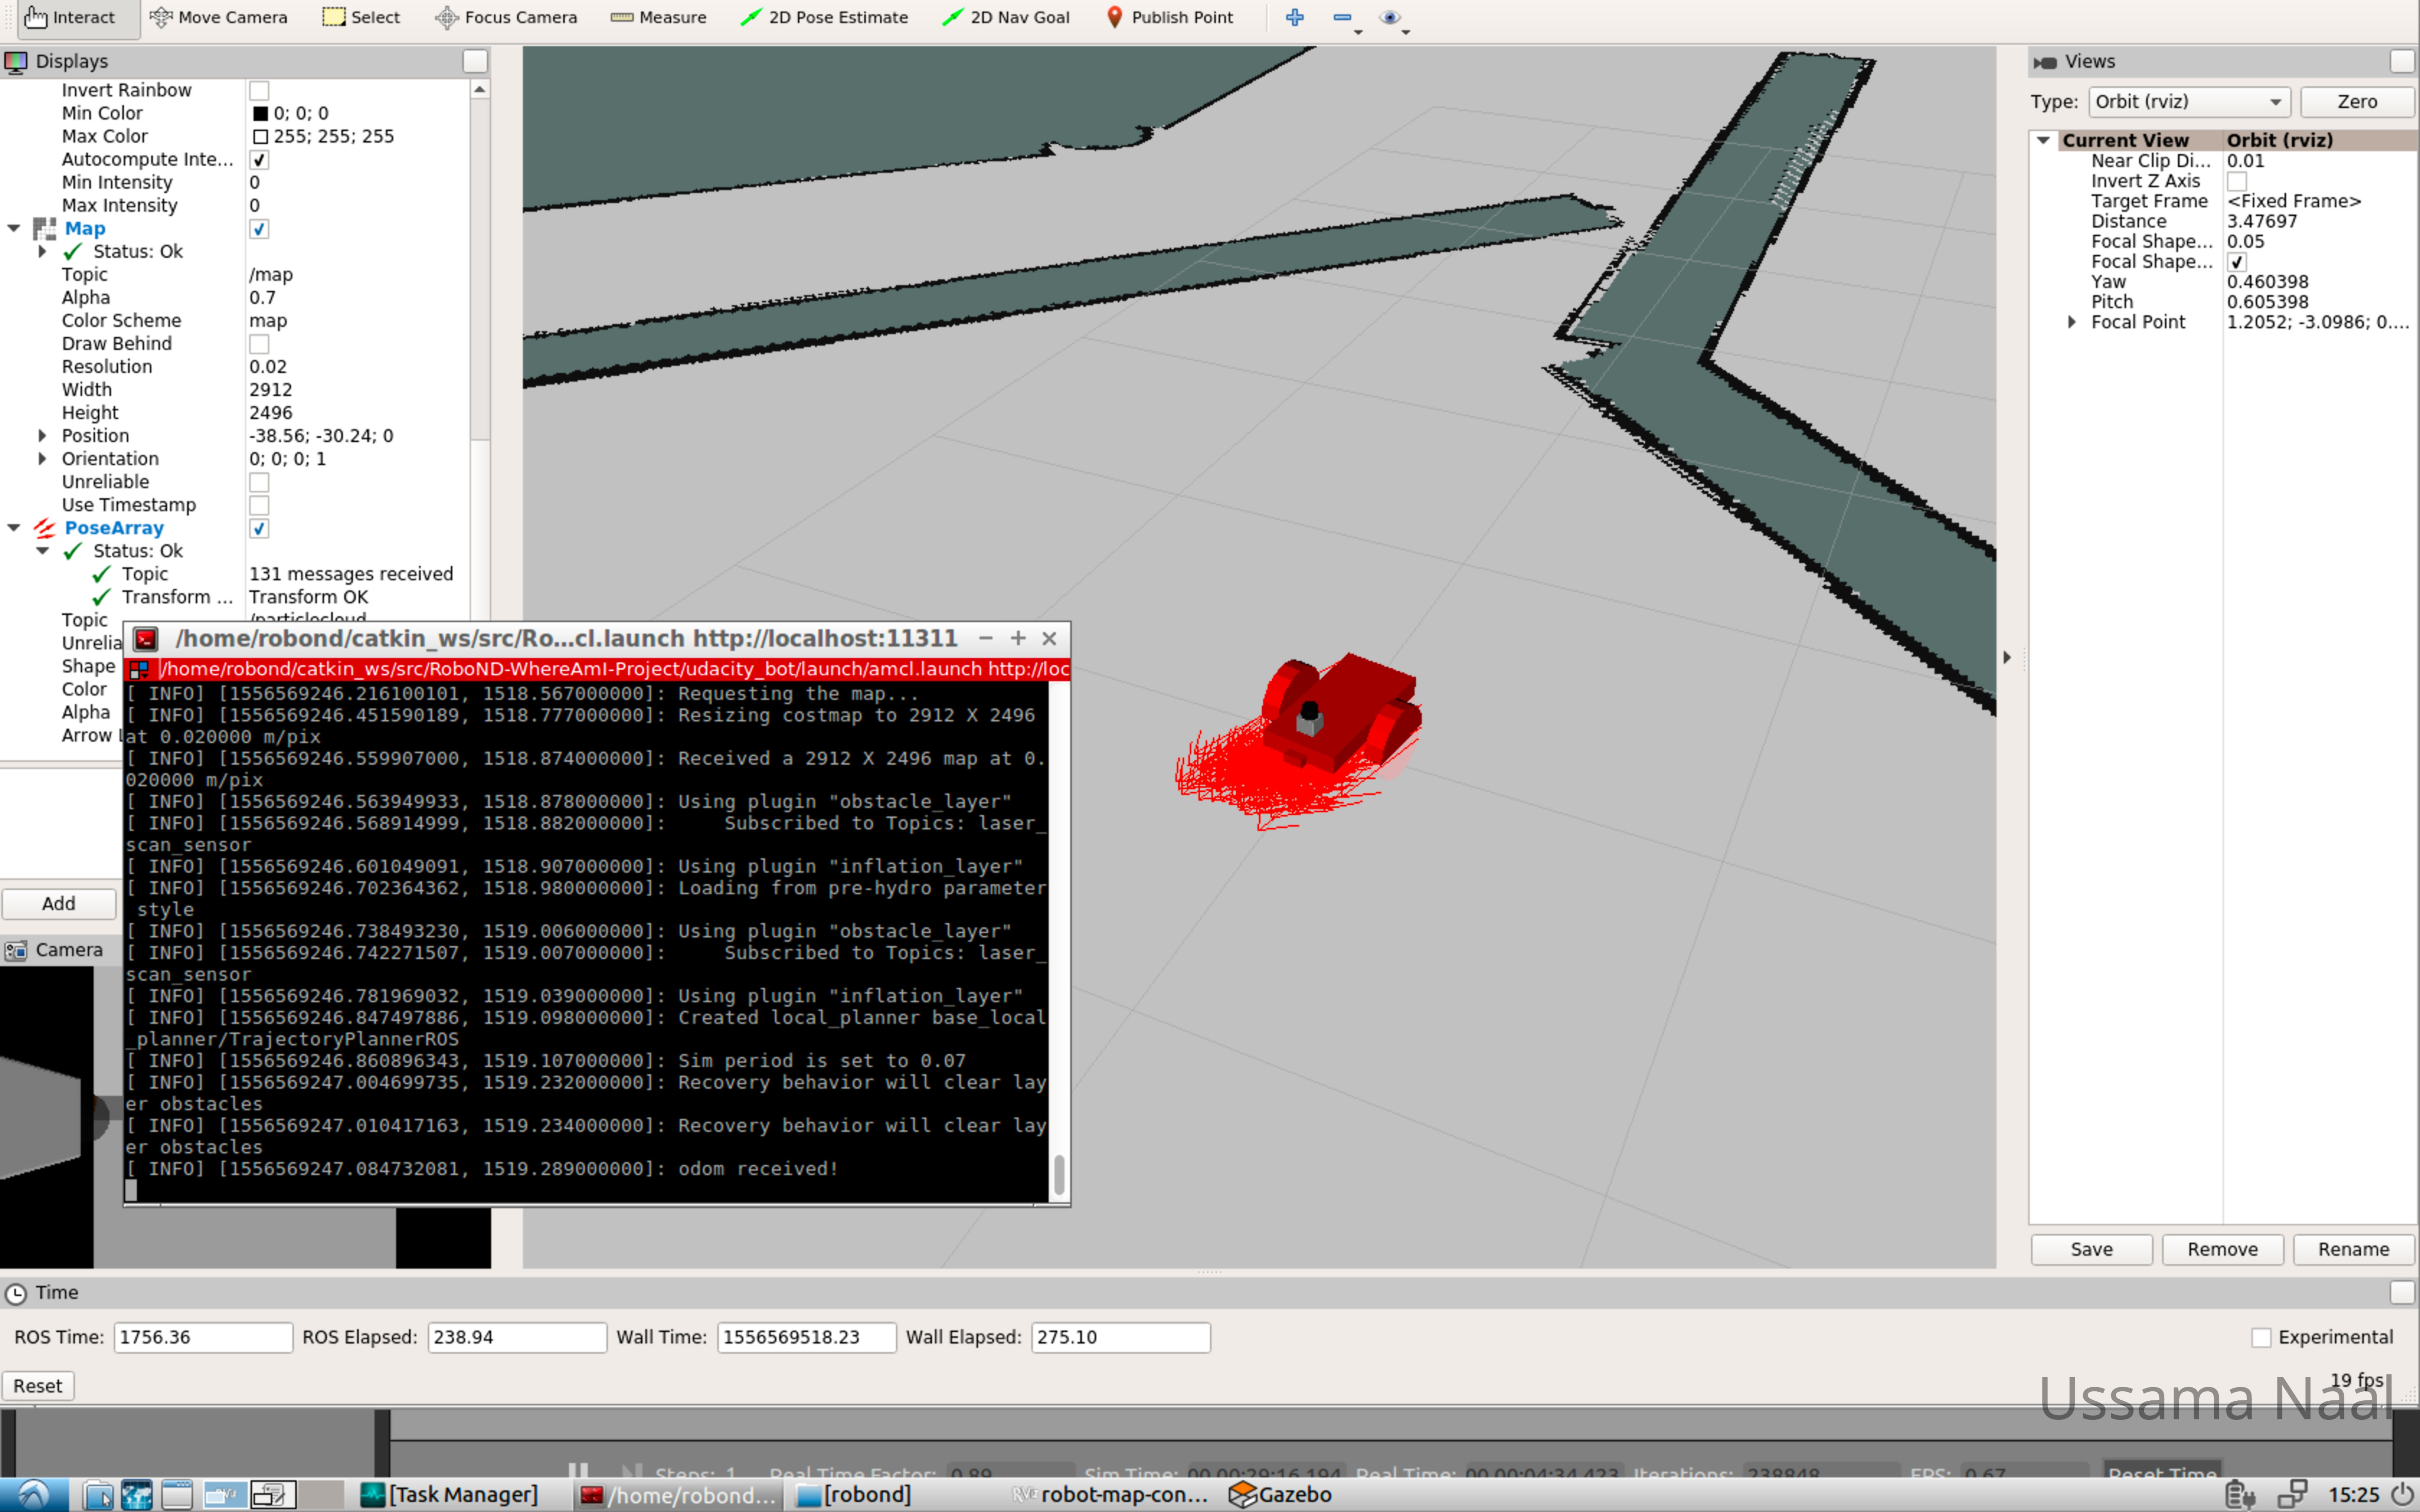
\includegraphics[width=\linewidth]{robot-at-goal.png}
      \caption{Robot at target location.}
      \label{fig:network-training}
\end{figure}

\section{Discussion}

The robot successfully manages to navigate to the target goal, however, there are still some occasions where the robot enters a stale state. That means there a possible room for improvement and parameter tuning to avoid going into such state.

Default MCL algorithm does not deal with kidnapped robot state. i.e. if the robot was moved to another spot on the map without being notified with change. The AMCL variant, however, can recover from this by continuously spawning few random samples from uniform distributed over the map.

Both MCL and AMCL can be used in scenarios where a given robot needs to localize and track its movement within a known map. Example of such uses are the Knightscope \cite{knightscope} autonomous security guard, where the robot constantly moving around to secure the perimeter of the protected site. Other examples are delivery robots with office or hotel spaces, vacuum cleaning robots, etc.

\section{Conclusion / Future work}

Further tune listed parameters and investigate the remaining list of parameters for the move\_base and AMCL packages.

Configure and run the system on actual robot.

Addition of other sensors such as RGB-D camera or a LIDAR would give better scan of the surrounding area of the robot and theoretically should improve localization accuracy. However, this would come at the cost of increased processing time, due to larger incoming data from the sensors. As mentioned in \cite{Fox99montecarlo} the responsiveness of the system is also important to successfully perform the localization. Because of that it would necessary to upgrade the system with better hardware for data processing like relying on GPUs. Luckily many hardware vendors are providing good options for GPUs specifically made  for on-board processing for the robot such as NVIDIA's Jetston X2 \cite{nvidia-jetston-x2}.

\bibliography{bib}
\bibliographystyle{ieeetr}

\end{document}